\documentclass[11pt,a4paper]{article}

\usepackage[utf8]{inputenc}
\usepackage[T1]{fontenc}
\usepackage[spanish,es-tabla,es-nodecimaldot]{babel}
\usepackage{lmodern}
\usepackage{microtype}
\usepackage[margin=2.5cm]{geometry}
\usepackage{graphicx}
\usepackage{booktabs}
\usepackage{float}
\usepackage{caption}
\usepackage{enumitem}
\usepackage{xcolor}
\usepackage{fancyhdr}
\usepackage[hidelinks]{hyperref}

\graphicspath{{figures/}}
\captionsetup{font=small,labelfont=bf}
\setlist{itemsep=2pt}
\definecolor{acento}{HTML}{1C5CAB}
\hypersetup{colorlinks=true,linkcolor=acento,urlcolor=acento,citecolor=acento}

\pagestyle{fancy}
\fancyhf{}
\fancyhead[L]{\small Reconocimiento de emociones en la voz}
\fancyhead[R]{\small Análisis exploratorio de RAVDESS}
\fancyfoot[C]{\thepage}

% Cifras generadas por notebooks/01_eda.ipynb
% Archivo generado automáticamente por notebooks/01_eda.ipynb -- no editar a mano
\newcommand{\nClips}{1440}
\newcommand{\nActores}{24}
\newcommand{\nEmociones}{8}
\newcommand{\nClipsNeutral}{96}
\newcommand{\nClipsOtras}{192}
\newcommand{\nEstereo}{5}
\newcommand{\tamanoMB}{590.3}
\newcommand{\durMedia}{3.7}
\newcommand{\durMin}{2.9}
\newcommand{\durMax}{5.3}
\newcommand{\durVozMedia}{1.9}
\newcommand{\silInicio}{0.937}
\newcommand{\silFinal}{0.893}
\newcommand{\fracSilencio}{49.8}
\newcommand{\foHombre}{149.3}
\newcommand{\foMujer}{256.9}
\newcommand{\rmsNormal}{0.009}
\newcommand{\rmsFuerte}{0.023}
\newcommand{\rmsRatio}{2.6}
\newcommand{\emoMaxRMS}{enojo}
\newcommand{\emoMinRMS}{calma}
\newcommand{\rmsMaxVal}{0.037}
\newcommand{\rmsMinVal}{0.004}
\newcommand{\emoMaxFo}{miedo}
\newcommand{\emoMinFo}{calma}
\newcommand{\foMaxVal}{270.7}
\newcommand{\foMinVal}{160.5}
\newcommand{\emoMaxDur}{asco}
\newcommand{\emoMinDur}{sorpresa}
\newcommand{\pcUno}{29.2}
\newcommand{\pcDos}{13.5}
\newcommand{\nPCNoventa}{15}
\newcommand{\nDescriptores}{30}
\newcommand{\frameLen}{2048}
\newcommand{\hopLen}{512}
\newcommand{\ventanaMs}{92.9}
\newcommand{\saltoMs}{23.2}
\newcommand{\nMujer}{720}
\newcommand{\nHombre}{720}
\newcommand{\atipTotalMujer}{120}
\newcommand{\atipTotalHombre}{111}
\newcommand{\atipMaxDesc}{RMS}
\newcommand{\kwTop}{Energía RMS media}
\newcommand{\kwTopEps}{0.446}
\newcommand{\kwLow}{Tasa de cruces por cero}
\newcommand{\kwLowEps}{0.117}
\newcommand{\tablaKruskal}{%
Energía RMS media & 645.5 & $<10^{-10}$ & 0.446 \\
Duración de voz (s) & 296.0 & $<10^{-10}$ & 0.202 \\
F0 media (Hz) & 290.9 & $<10^{-10}$ & 0.198 \\
Centroide espectral (Hz) & 248.3 & $<10^{-10}$ & 0.169 \\
Rango de F0 p5–p95 (Hz) & 239.7 & $<10^{-10}$ & 0.162 \\
Tasa de cruces por cero & 174.4 & $<10^{-10}$ & 0.117 \\
}
\newcommand{\tablaMedianas}{%
neutral & 1.63 & 0.006 & 0.104 & 2056 & 177 \\
calma & 1.95 & 0.004 & 0.114 & 2220 & 161 \\
alegría & 1.72 & 0.019 & 0.113 & 2250 & 239 \\
tristeza & 1.82 & 0.007 & 0.116 & 2192 & 203 \\
enojo & 1.89 & 0.037 & 0.140 & 2544 & 262 \\
miedo & 1.68 & 0.024 & 0.125 & 2527 & 271 \\
asco & 2.04 & 0.010 & 0.138 & 2476 & 199 \\
sorpresa & 1.60 & 0.016 & 0.122 & 2407 & 265 \\
}
\newcommand{\tablaAtipicos}{%
ZCR & 11 & 1.5\,\% & 17 & 2.4\,\% \\
RMS & 75 & 10.4\,\% & 75 & 10.4\,\% \\
MFCC1 & 0 & 0.0\,\% & 1 & 0.1\,\% \\
MFCC2 & 13 & 1.8\,\% & 9 & 1.2\,\% \\
MFCC3 & 12 & 1.7\,\% & 3 & 0.4\,\% \\
MFCC4 & 9 & 1.2\,\% & 6 & 0.8\,\% \\
}
\newcommand{\tablaFrameHop}{%
512 & 128 & 23.2 & 5.8 & 431 \\
1024 & 256 & 46.4 & 11.6 & 216 \\
2048 & 512 & 92.9 & 23.2 & 108 \\
4096 & 1024 & 185.8 & 46.4 & 54 \\
}


\title{\textbf{Reconocimiento de emociones en la voz}\\[4pt]
\large Análisis exploratorio del corpus RAVDESS (habla)}
\author{Saúl Ubaldo Rojas Vázquez \and Karols Cisneros \and Mónica}
\date{\today}

\begin{document}
\maketitle
\thispagestyle{empty}

\begin{abstract}
\noindent Se presenta el análisis exploratorio del subconjunto de habla del corpus RAVDESS
(\nClips{} grabaciones, \nActores{} actores, \nEmociones{} emociones) como etapa previa a la construcción
de un clasificador de emociones a partir de la señal de voz. Los datos se alojaron en Supabase
(Storage + PostgreSQL) para consumirlos sin mantener copias locales. Se verificó la calidad de los
datos, se caracterizó la composición del corpus y se extrajeron \nDescriptores{} descriptores acústicos por
clip (energía, tasa de cruces por cero, centroide y \emph{roll-off} espectral, frecuencia fundamental y
MFCC). Todos los descriptores difieren significativamente entre emociones (Kruskal--Wallis, $p<10^{-10}$);
la energía RMS es el más discriminante ($\varepsilon^2=\kwTopEps$). Los valores atípicos se concentran en
la energía (\(\approx\)10\,\% de los clips por género) y provienen de emociones de alta activación, y los
gráficos de radar muestran perfiles por emoción muy parecidos en mujeres y hombres. Sin embargo, las proyecciones en baja
dimensión muestran que la estructura dominante de los datos corresponde al \emph{hablante} (en particular
a su género) y no a la emoción, lo que condiciona el diseño del modelo y su protocolo de evaluación.
\end{abstract}

\section{Introducción y objetivos}

El reconocimiento automático de emociones en la voz (\emph{Speech Emotion Recognition}, SER) busca inferir
el estado afectivo de un hablante a partir de propiedades acústicas de su señal, como la intensidad, el
tono o el timbre. Como referencia para la etapa de modelado se toma el enfoque de \cite{kaggleref}, basado en
MFCC, ZCR y energía con una red convolucional 1D. Antes de entrenar un modelo es necesario entender qué contiene el corpus, qué tan
balanceado está y qué propiedades acústicas separan realmente a las emociones.

\paragraph{Objetivo general.} Caracterizar el corpus RAVDESS (habla) para fundamentar el diseño de un
modelo de clasificación de emociones a partir de la voz.

\paragraph{Objetivos específicos.}
\begin{enumerate}[label=\arabic*.]
  \item Publicar el corpus en Supabase para su consumo remoto, sin depender de archivos locales.
  \item Verificar la integridad y la calidad de los datos (duplicados, formatos, canales, duraciones).
  \item Describir la composición del corpus por emoción, intensidad, género y actor.
  \item Extraer descriptores acústicos interpretables y evaluar cuáles distinguen entre emociones.
  \item Identificar fuentes de variación ajenas a la emoción (hablante, género, intensidad) que deban
        controlarse durante el modelado.
\end{enumerate}

\section{Dataset}

\subsection{Descripción}

RAVDESS (\emph{Ryerson Audio-Visual Database of Emotional Speech and Song}) \cite{livingstone2018} contiene
grabaciones de \nActores{} actores profesionales (12 hombres y 12 mujeres) con acento norteamericano neutro.
Se usó la copia publicada en Kaggle (\texttt{orvile/ravdess-dataset}), que incluye audio y video de habla y
canto (\(\approx\)24\,GB). Para este trabajo se tomó únicamente el \textbf{audio de habla}
(\texttt{Audio\_Speech\_Actors\_01-24}): \nClips{} archivos WAV a 48\,kHz y 16 bits, \tamanoMB{}\,MB.

Cada actor pronuncia dos frases léxicamente neutras, \emph{``Kids are talking by the door''} y
\emph{``Dogs are sitting by the door''}, con ocho emociones: neutral, calma, alegría, tristeza, enojo,
miedo, asco y sorpresa. Todas salvo neutral se graban con intensidad normal y fuerte, y cada combinación
se repite dos veces, es decir, $2\times2\times(7\times2+1)=60$ clips por actor.

\subsection{Codificación de los archivos}

Los metadatos están codificados en el nombre del archivo, \texttt{MM-CC-EE-II-SS-RR-AA.wav}
(Tabla~\ref{tab:codigo}). Por ejemplo, \texttt{03-01-05-02-01-01-07.wav} es audio de habla, enojo, intensidad
fuerte, frase ``Kids'', primera repetición, actor 7 (hombre).

\begin{table}[H]
\centering
\caption{Campos del nombre de archivo de RAVDESS.}
\label{tab:codigo}
\small
\begin{tabular}{@{}llp{8.2cm}@{}}
\toprule
Campo & Código & Valores \\
\midrule
Modalidad   & MM & 01 audio-video, 02 solo video, \textbf{03 solo audio} \\
Canal vocal & CC & \textbf{01 habla}, 02 canto \\
Emoción     & EE & 01 neutral, 02 calma, 03 alegría, 04 tristeza, 05 enojo, 06 miedo, 07 asco, 08 sorpresa \\
Intensidad  & II & 01 normal, 02 fuerte (neutral solo tiene normal) \\
Frase       & SS & 01 ``Kids are talking by the door'', 02 ``Dogs are sitting by the door'' \\
Repetición  & RR & 01, 02 \\
Actor       & AA & 01--24; impar = hombre, par = mujer \\
\bottomrule
\end{tabular}
\end{table}

\subsection{Almacenamiento en Supabase}

Para no depender de copias locales, el corpus se publicó en el proyecto Supabase
\texttt{ser-voz-emocional}:
\begin{itemize}
  \item \textbf{Storage}: bucket público \texttt{ravdess-audio} con los \nClips{} WAV, organizados como
        \texttt{Actor\_XX/<archivo>.wav}.
  \item \textbf{Base de datos}: tabla \texttt{public.ravdess\_clips} con una fila por clip (nombre, ruta en
        Storage, actor, género, emoción, intensidad, frase, repetición, tamaño, frecuencia de muestreo,
        canales y duración).
  \item \textbf{Seguridad}: \emph{Row Level Security} activo; los roles públicos solo tienen permiso de
        lectura. Los permisos de escritura usados durante la carga se eliminaron al terminar.
\end{itemize}
Tras la carga se verificó que los \nClips{} objetos de Storage coinciden uno a uno con las filas de la
tabla y que el tamaño total coincide con el de la fuente. Los notebooks leen los metadatos vía la API REST
y descargan los audios bajo demanda a una caché temporal.

\section{Metodología del análisis exploratorio}

\begin{enumerate}[label=\arabic*.]
  \item \textbf{Calidad de datos}: búsqueda de duplicados y nulos; revisión de frecuencia de muestreo,
        número de canales y duración.
  \item \textbf{Preprocesamiento}: remuestreo a 22\,050\,Hz, conversión a mono y recorte de silencios
        iniciales y finales (umbral de 30\,dB bajo el pico).
  \item \textbf{Parámetros de cuadro}: \emph{frame length} de \frameLen{} muestras (\ventanaMs\,ms) y
        \emph{hop length} de \hopLen{} muestras (\saltoMs\,ms), justificados en la
        Sección~\ref{sec:framehop}.
  \item \textbf{Descriptores por clip} (sobre la señal sin silencios): energía RMS (media y desviación),
        tasa de cruces por cero (ZCR), centroide y \emph{roll-off} espectral, frecuencia fundamental F0
        estimada con pYIN (media, desviación y rango p5--p95), fracción de cuadros sonoros y 20 MFCC
        promediados en el tiempo \cite{mcfee2015}.
  \item \textbf{Pruebas estadísticas}: Kruskal--Wallis entre las ocho emociones con tamaño de efecto
        $\varepsilon^2=(H-k+1)/(n-k)$; comparación de medianas por género e intensidad.
  \item \textbf{Valores atípicos}: regla IQR ($x<Q_1-1.5\,\mathrm{IQR}$ o $x>Q_3+1.5\,\mathrm{IQR}$) sobre
        ZCR, RMS y MFCC~1--4, con cuartiles calculados dentro de cada género.
  \item \textbf{Patrones por emoción}: gráficos de radar con la media de cada descriptor por emoción,
        normalizada con Min-Max entre emociones dentro de cada género.
  \item \textbf{Proyecciones}: PCA y t-SNE sobre los descriptores estandarizados.
\end{enumerate}

\subsection{Longitud de cuadro y salto}
\label{sec:framehop}

Las tres familias de características que usa el modelo de referencia \cite{kaggleref} (MFCC, ZCR y RMS) se
extraen con librosa \cite{mcfee2015} cuadro a cuadro. Antes hay que fijar dos parámetros: el
\emph{frame length}, que es el número de muestras de cada cuadro, y el \emph{hop length}, que es cuánto
avanza la ventana entre un cuadro y el siguiente. Cuadros más largos mejoran la resolución en frecuencia
pero suavizan los cambios rápidos; un salto menor da más resolución temporal a cambio de más cuadros.

La Tabla~\ref{tab:framehop} y la Figura~\ref{fig:framehop} comparan cuatro combinaciones con 75\,\% de
traslape. Con 512 muestras (23\,ms) la ZCR es muy ruidosa. Con 4096 (186\,ms) se pierden los picos de
energía de cada sílaba. La combinación \frameLen/\hopLen{} (\ventanaMs/\saltoMs\,ms) conserva la forma
silábica de la envolvente con curvas estables. Además es el valor por defecto de librosa y el que usa la
referencia, y produce 108 cuadros en una ventana de 2.5\,s.

\begin{table}[H]
\centering
\caption{Combinaciones de \emph{frame length} y \emph{hop length} evaluadas (22\,050\,Hz).}
\label{tab:framehop}
\small
\begin{tabular}{@{}rrrrr@{}}
\toprule
Frame (muestras) & Hop (muestras) & Ventana (ms) & Salto (ms) & Cuadros en 2.5\,s \\
\midrule
\tablaFrameHop
\bottomrule
\end{tabular}
\end{table}

\begin{figure}[H]
\centering
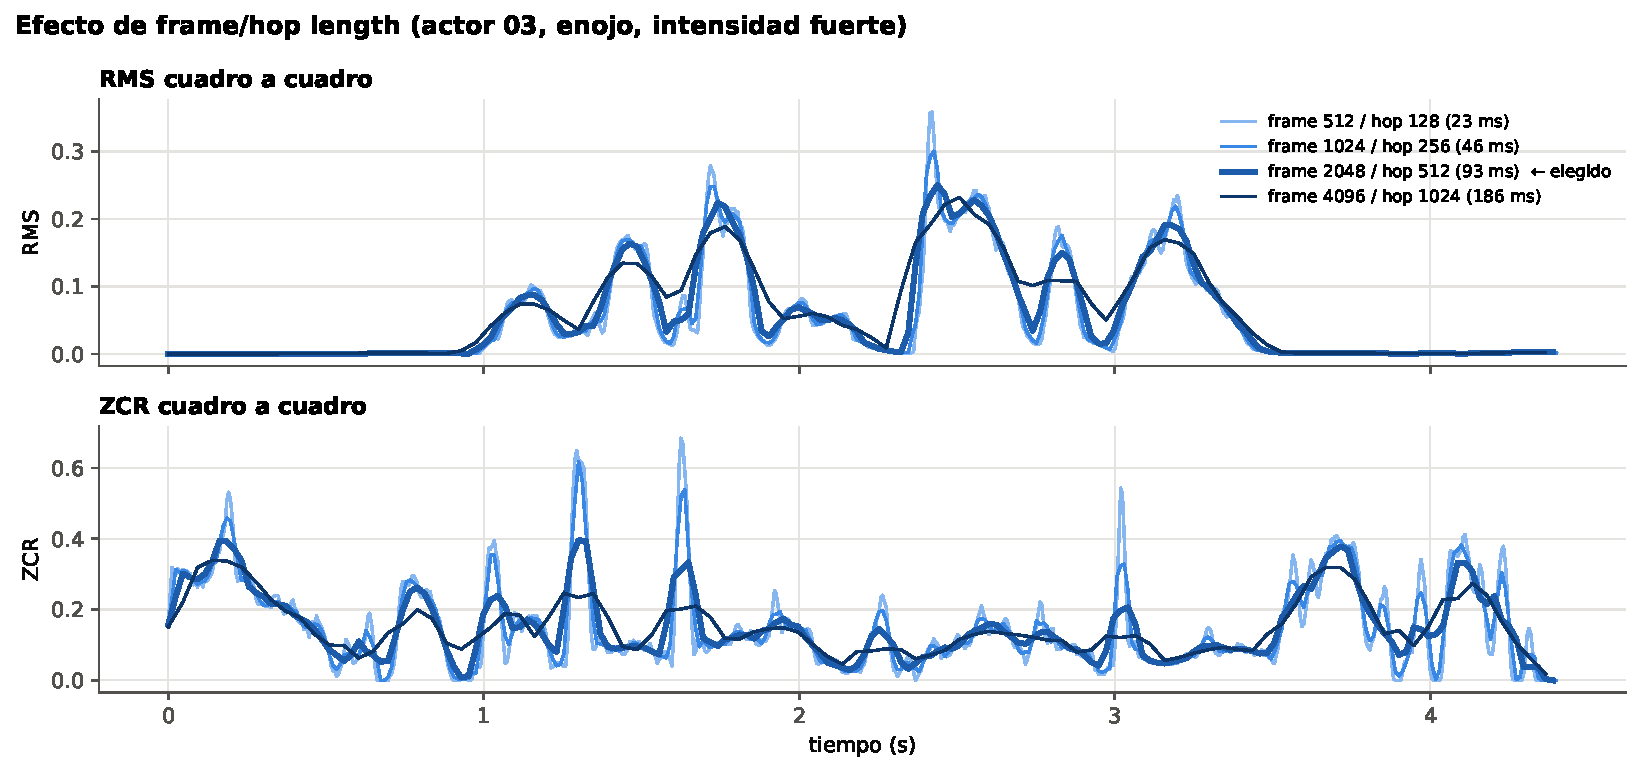
\includegraphics[width=\linewidth]{frame_hop_length}
\caption{RMS y ZCR cuadro a cuadro de un mismo clip con distintas longitudes de cuadro; la línea gruesa
es la combinación elegida.}
\label{fig:framehop}
\end{figure}

\section{Resultados del análisis exploratorio}

\subsection{Calidad de los datos}

No hay valores nulos ni archivos duplicados, y los \nClips{} archivos esperados por el diseño factorial
están presentes. Todos están muestreados a 48\,kHz, pero \nEstereo{} clips están en estéreo, por lo que se
convierten a mono durante la carga. La duración de los clips va de \durMin{} a \durMax{}\,s
(media \durMedia{}\,s).

\subsection{Composición del corpus}

El diseño es perfectamente balanceado por actor (60 clips cada uno) y por género (720 clips por género).
La única asimetría está en la emoción neutral, que tiene \nClipsNeutral{} clips frente a \nClipsOtras{} del
resto, porque no se graba con intensidad fuerte (Figura~\ref{fig:dist}). Esto genera un desbalance
moderado de 1:2 que debe considerarse al entrenar (pesos por clase o métricas macro) y al interpretar la
exactitud por clase.

\begin{figure}[H]
\centering
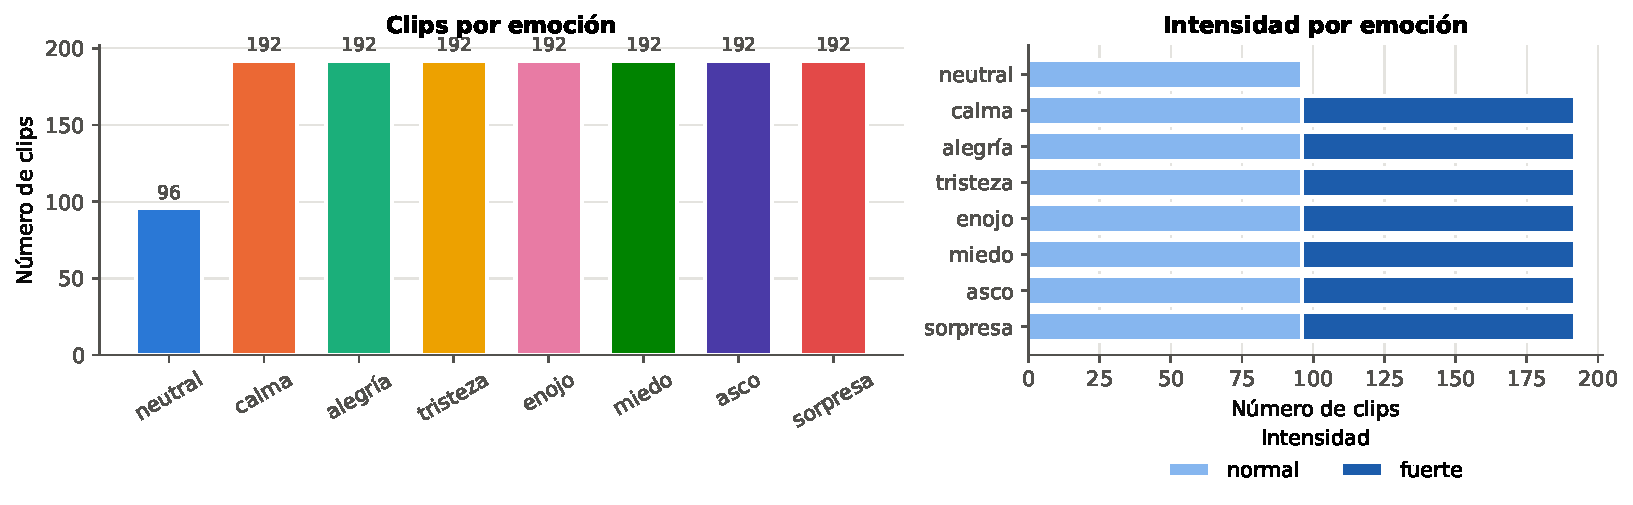
\includegraphics[width=\linewidth]{distribucion_emociones}
\caption{Número de clips por emoción y su desglose por intensidad. Neutral solo tiene intensidad normal.}
\label{fig:dist}
\end{figure}

\subsection{Duración y silencios}

En promedio, cerca de la mitad de cada clip (\fracSilencio\,\%) es silencio: \silInicio\,s al inicio y
\silFinal\,s al final. La voz efectiva dura \durVozMedia\,s en promedio. Las emociones difieren
ligeramente en duración: \emoMaxDur{} produce las emisiones más largas y \emoMinDur{} las más cortas
(Figura~\ref{fig:dur}). Por ello conviene recortar silencios o usar una ventana fija alineada con la voz
antes de extraer características, ya que de lo contrario el modelo aprende sobre segmentos vacíos.

\begin{figure}[H]
\centering
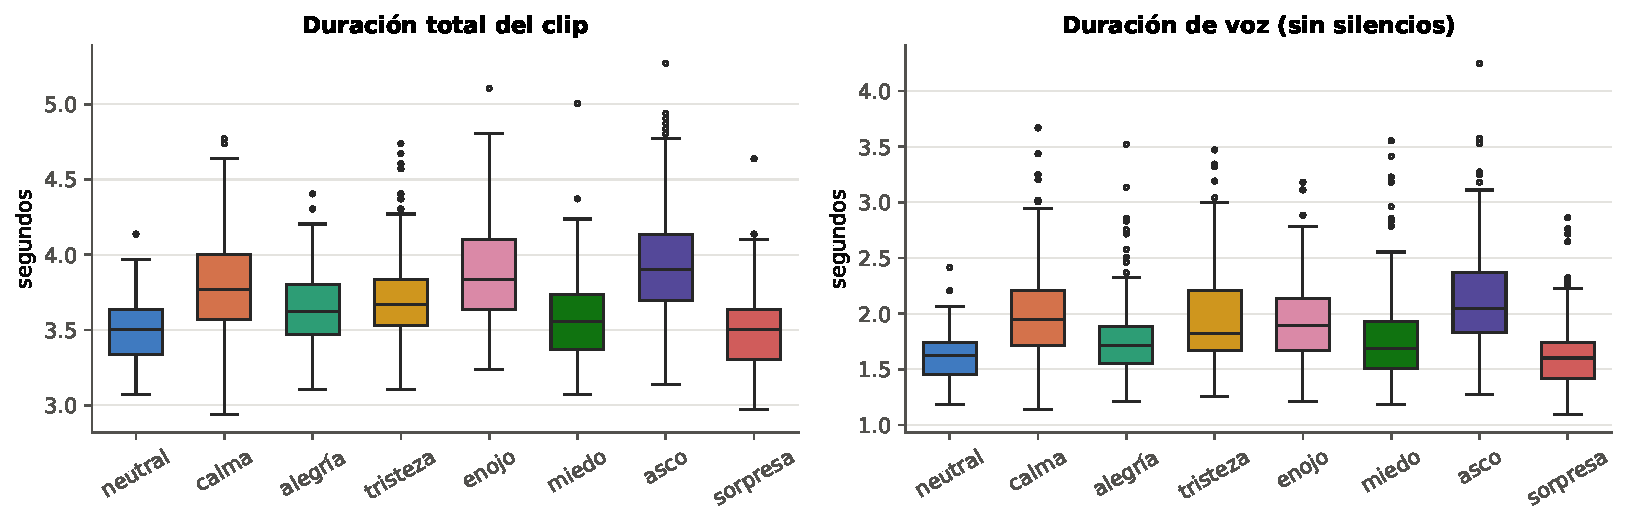
\includegraphics[width=\linewidth]{duraciones}
\caption{Duración total del clip y duración de la voz tras recortar silencios, por emoción.}
\label{fig:dur}
\end{figure}

\subsection{Forma de onda (\emph{waveplot}) y espectrograma}

La Figura~\ref{fig:ondas} muestra el \emph{waveplot} de la misma frase para cada emoción, dicha por una
mujer (actor 04) y un hombre (actor 03). En ambos, enojo, alegría y miedo tienen mayor amplitud y
envolventes más abruptas, mientras que neutral y calma son de baja energía. Asco varía entre hablantes:
la actriz lo produce con más energía que el actor. En los espectrogramas (Figura~\ref{fig:espec}), las emociones de alta activación concentran más
energía en frecuencias altas y muestran armónicos más espaciados, es decir, un tono más agudo.

\begin{figure}[H]
\centering
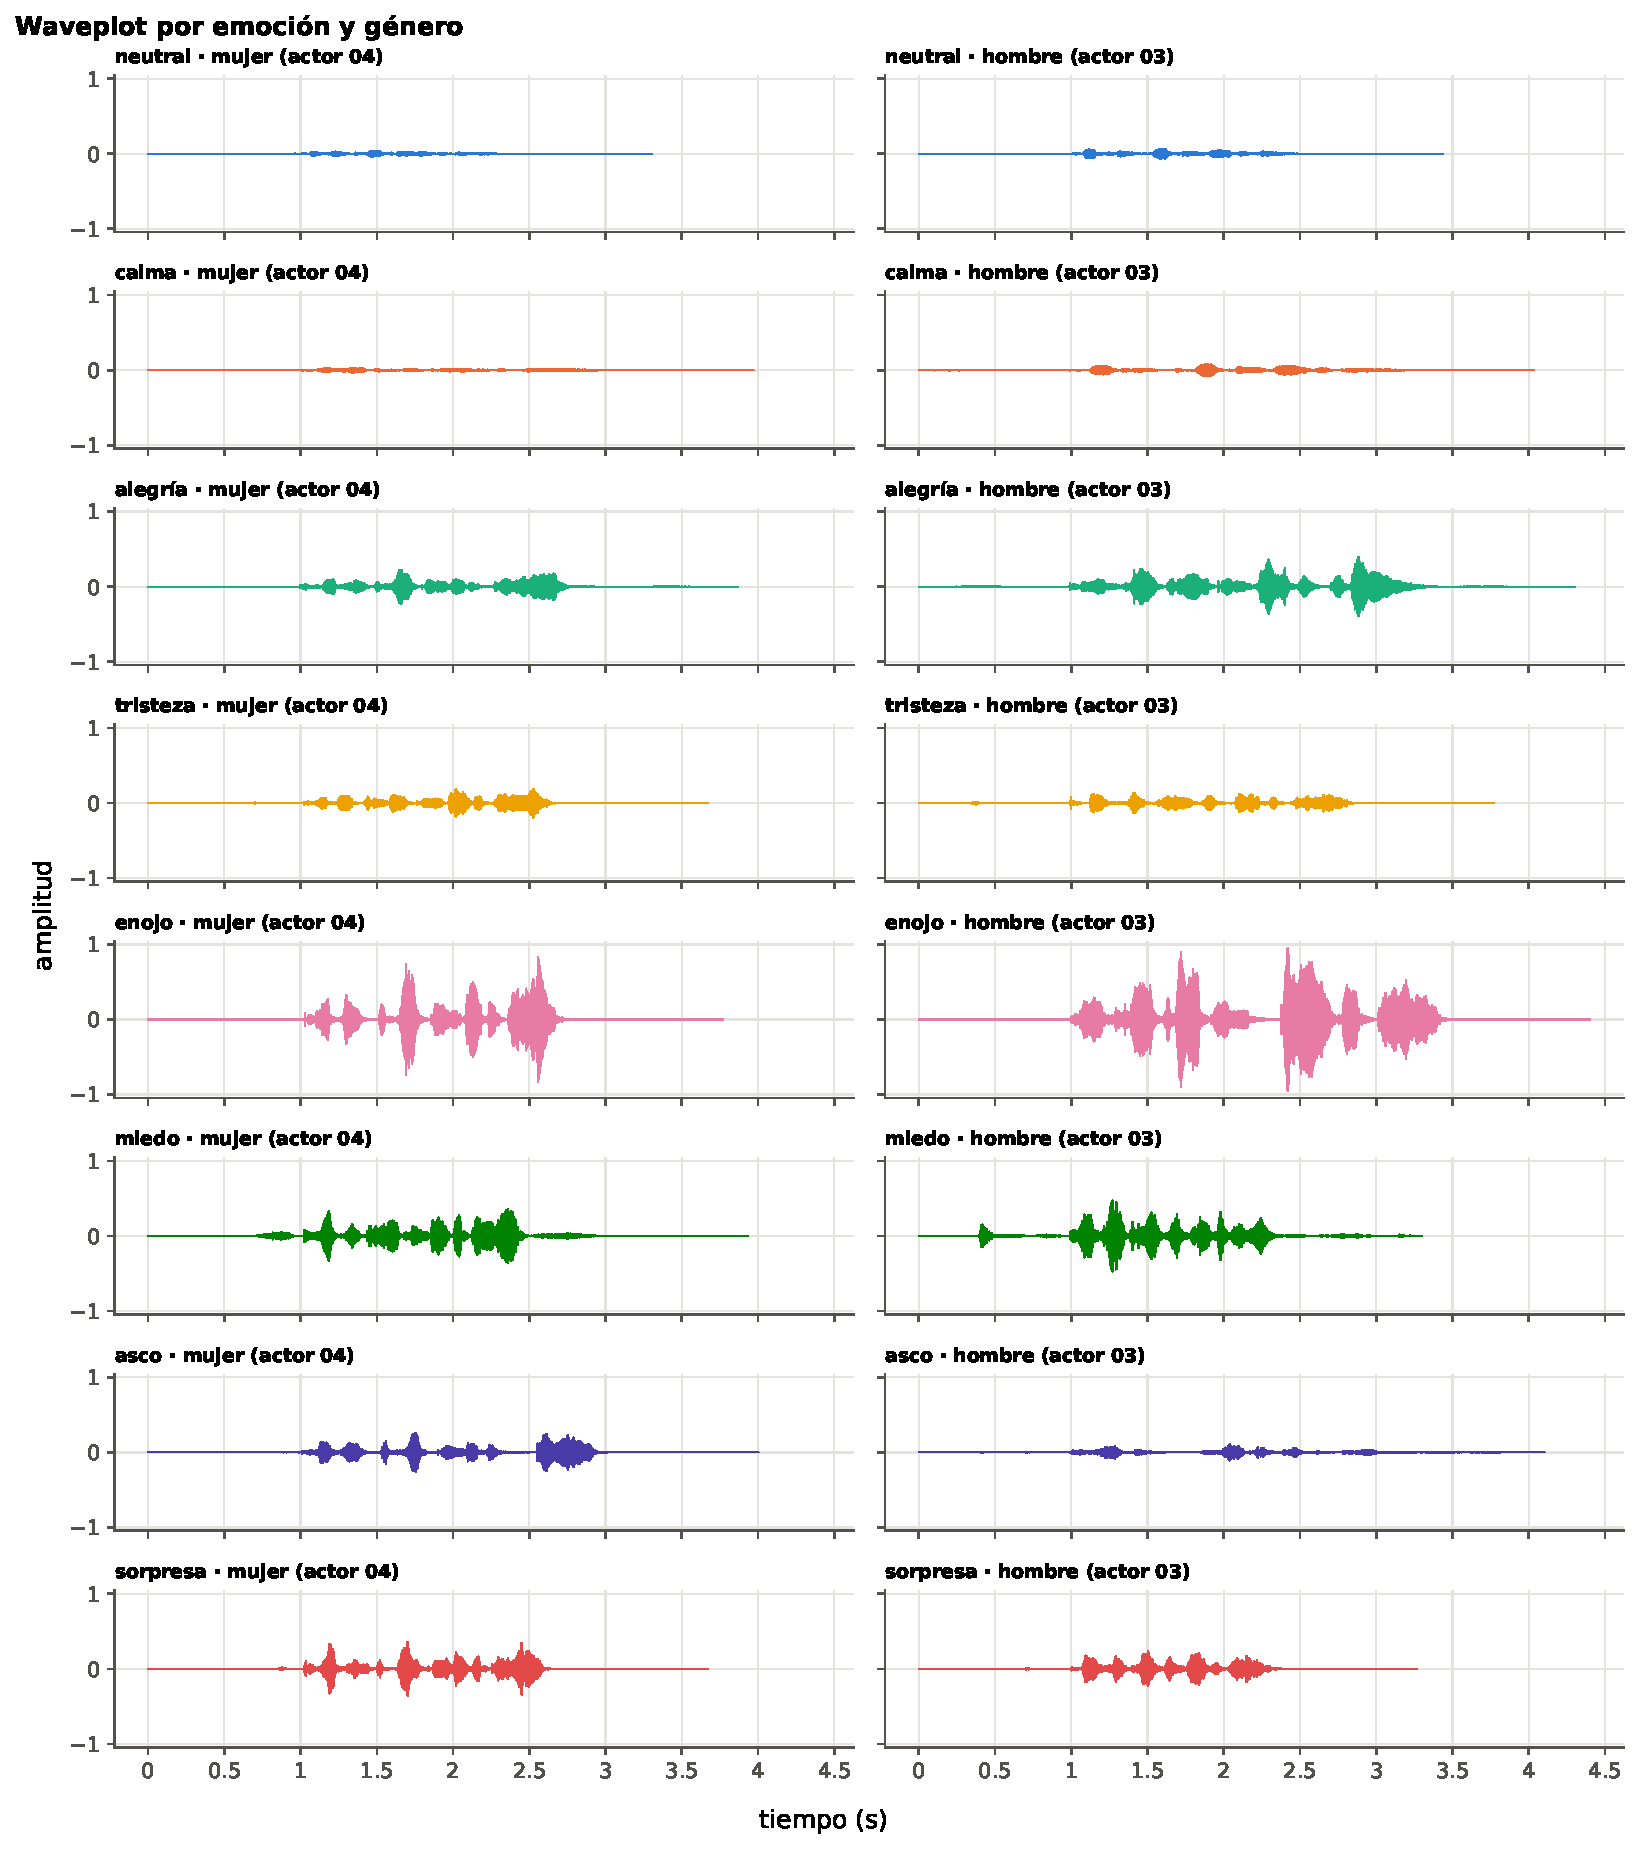
\includegraphics[width=.95\linewidth]{ondas_por_emocion}
\caption{\emph{Waveplot} por emoción y género: frase ``Kids are talking by the door'', repetición 1,
intensidad fuerte (normal en neutral).}
\label{fig:ondas}
\end{figure}

Para ver el patrón más allá de un solo hablante, la Figura~\ref{fig:envolvente} resume la envolvente RMS
de los \nClips{} clips. La voz empieza alrededor del segundo 1 en todas las emociones, lo que confirma el
silencio inicial. Enojo tiene un ataque marcado al inicio de la frase y la energía más alta durante toda
la emisión, seguido por miedo y alegría. Neutral, calma y tristeza quedan por debajo de la mediana global.
Asco se extiende hasta cerca del segundo 3, mientras que sorpresa termina antes.

\begin{figure}[H]
\centering
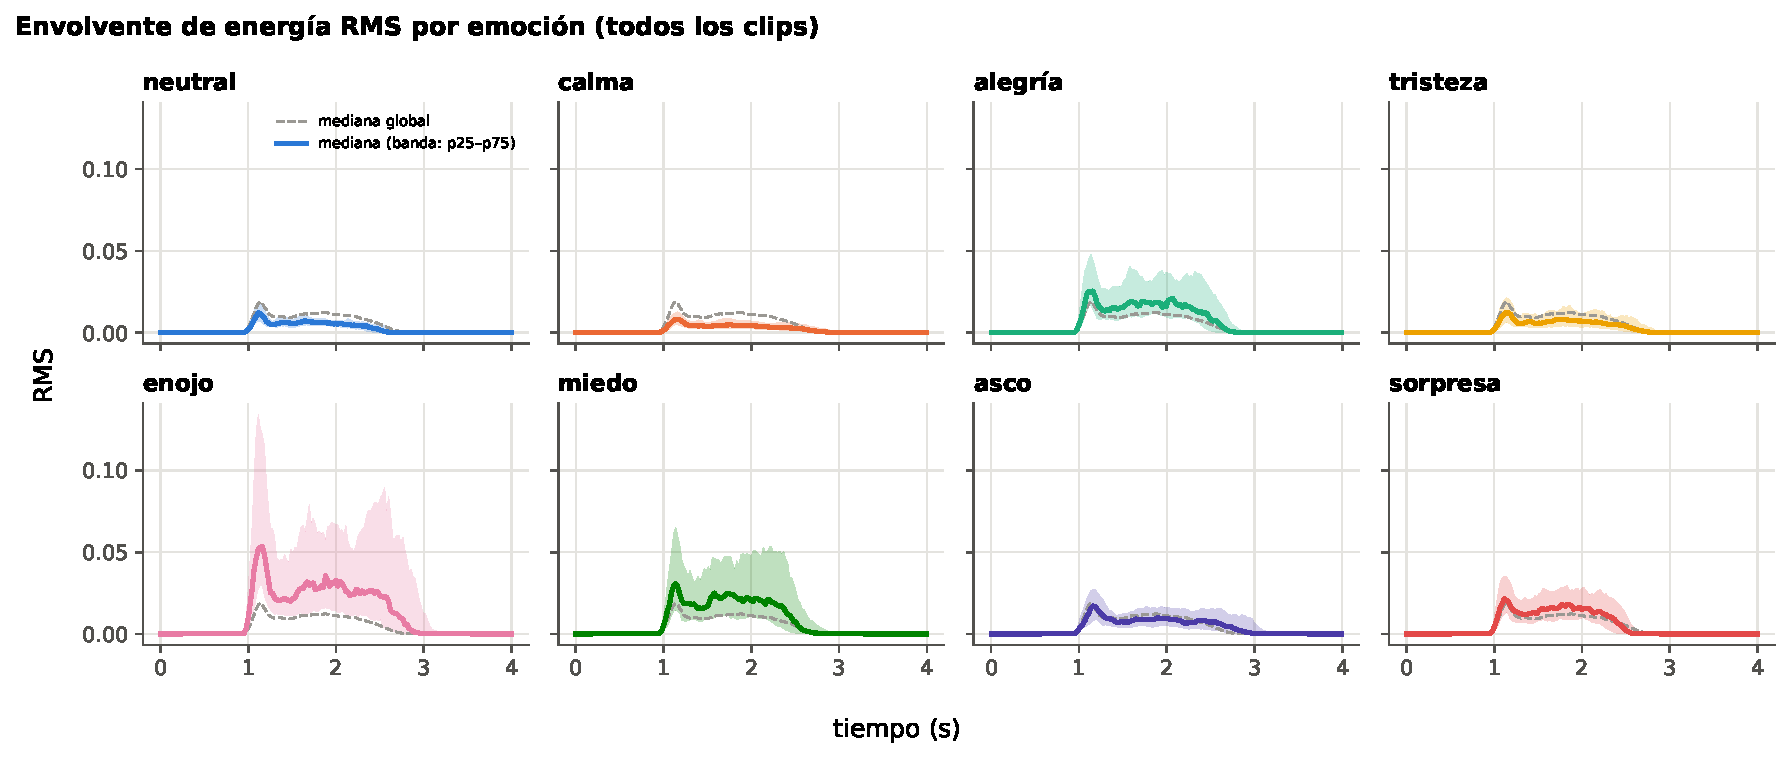
\includegraphics[width=\linewidth]{envolvente_rms_por_emocion}
\caption{Envolvente RMS por emoción: mediana (línea) y rango intercuartílico (banda) de todos los clips;
la línea punteada es la mediana global.}
\label{fig:envolvente}
\end{figure}

\begin{figure}[H]
\centering
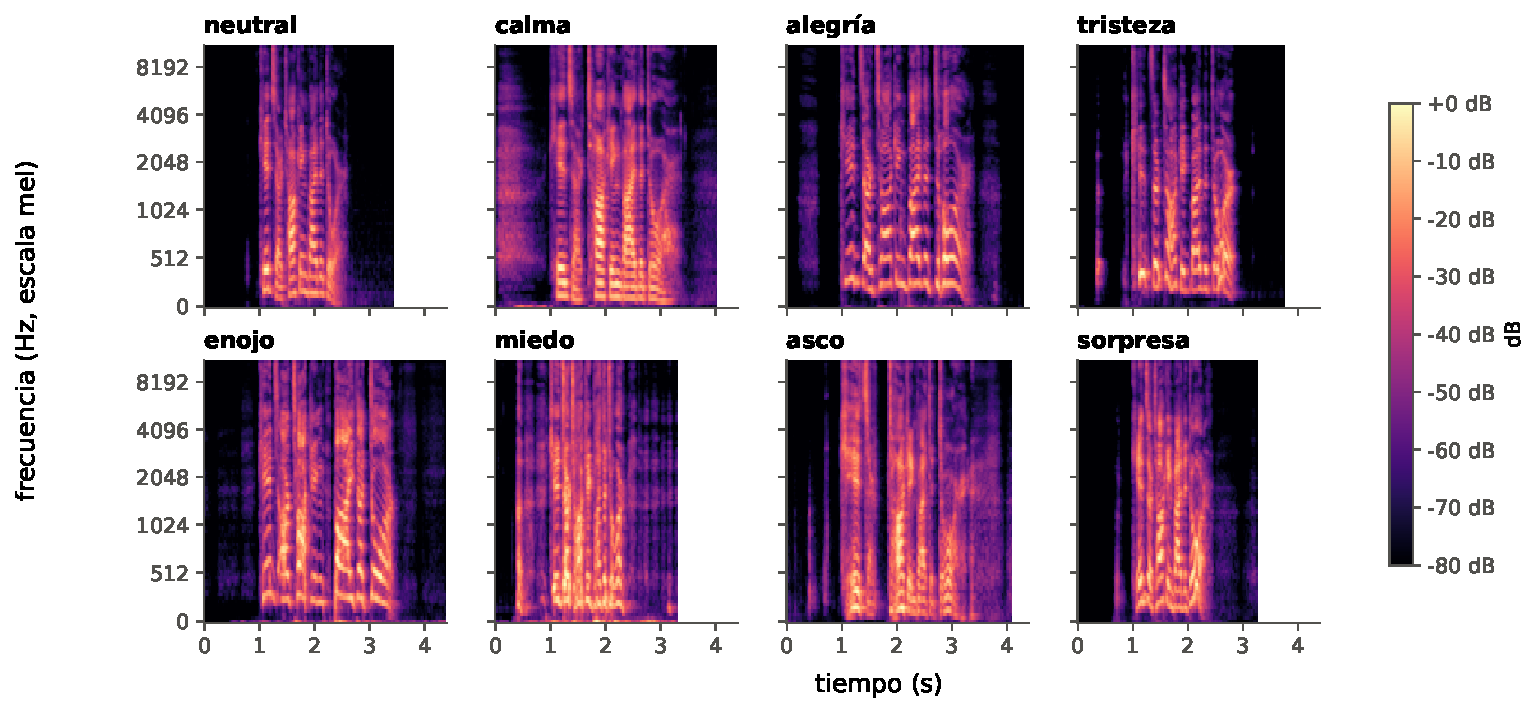
\includegraphics[width=\linewidth]{espectrogramas_por_emocion}
\caption{Espectrogramas mel por emoción (actor 03).}
\label{fig:espec}
\end{figure}

\subsection{Descriptores acústicos por emoción}

La Tabla~\ref{tab:medianas} y la Figura~\ref{fig:desc} resumen los descriptores principales. La energía
RMS es la variable que más cambia: \emoMaxRMS{} alcanza una mediana de \rmsMaxVal{} frente a \rmsMinVal{}
en \emoMinRMS. La F0 media sigue un patrón similar, más alta en \emoMaxFo{} (\foMaxVal\,Hz) y más baja en
\emoMinFo{} (\foMinVal\,Hz). El centroide espectral separa a las emociones de alta activación (enojo,
miedo, asco) de las de baja activación (neutral, calma).

\begin{table}[H]
\centering
\caption{Mediana de los descriptores por emoción (señal sin silencios).}
\label{tab:medianas}
\small
\begin{tabular}{@{}lrrrrr@{}}
\toprule
Emoción & Dur. voz (s) & RMS & ZCR & Centroide (Hz) & F0 (Hz) \\
\midrule
\tablaMedianas
\bottomrule
\end{tabular}
\end{table}

\begin{figure}[H]
\centering
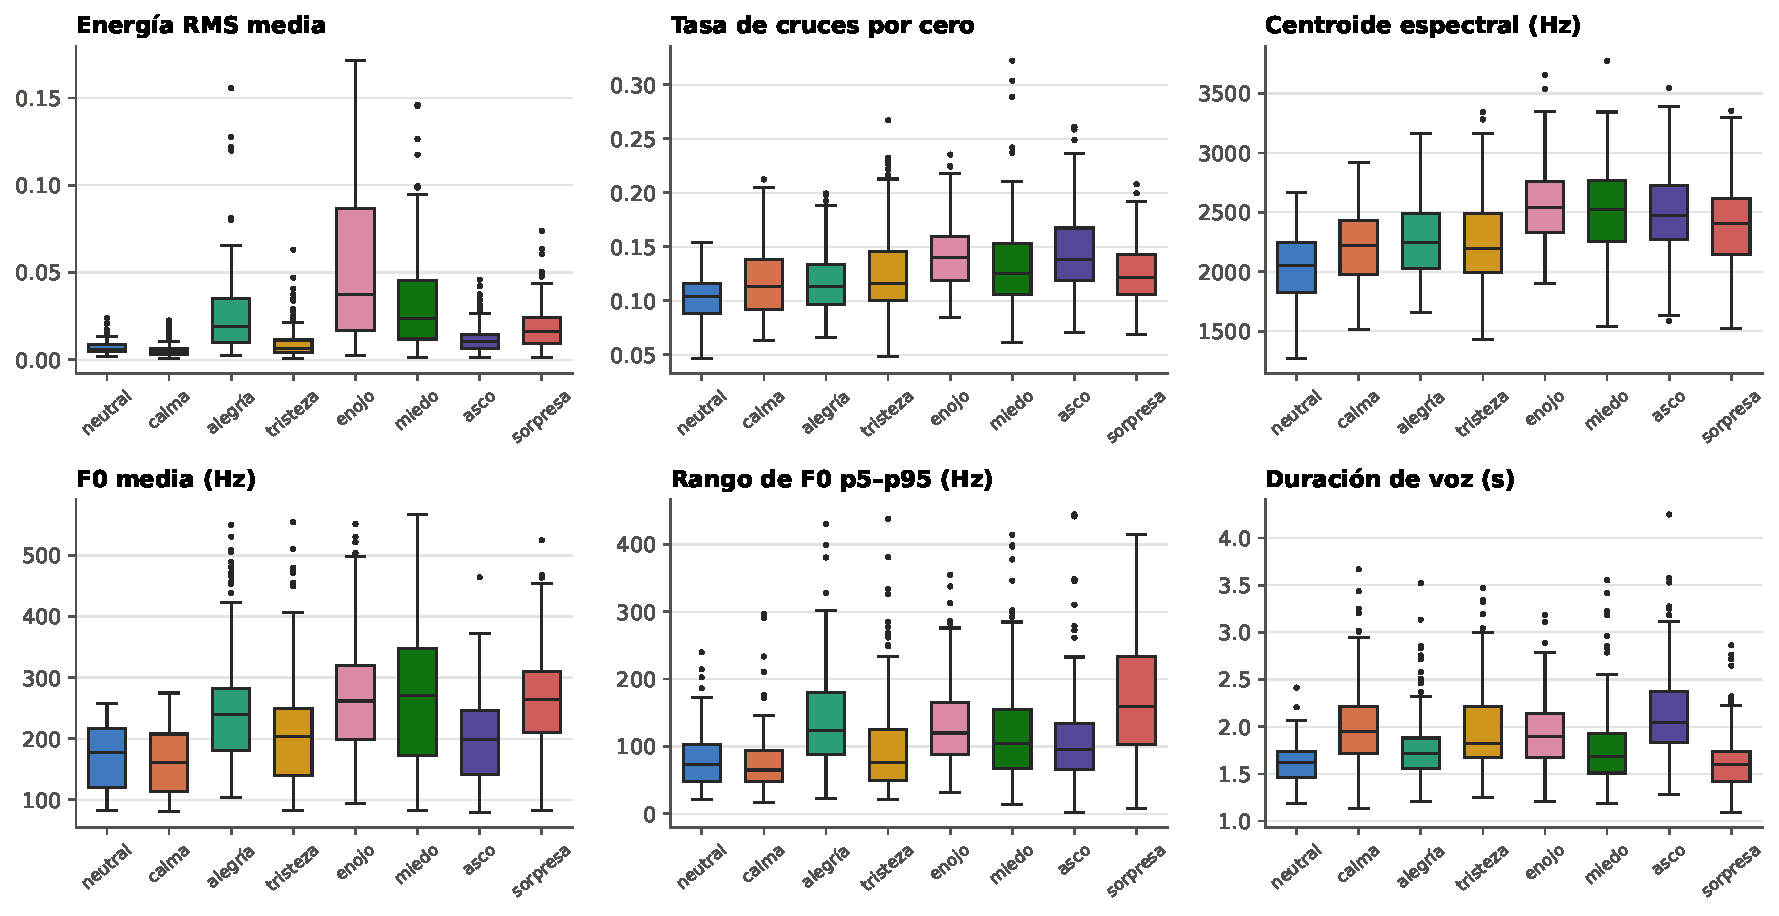
\includegraphics[width=\linewidth]{descriptores_por_emocion}
\caption{Distribución de seis descriptores acústicos por emoción.}
\label{fig:desc}
\end{figure}

Según la prueba de Kruskal--Wallis, los seis descriptores difieren significativamente entre emociones
(Tabla~\ref{tab:kw}). El tamaño de efecto indica que la energía (\kwTop, $\varepsilon^2=\kwTopEps$) es el
descriptor más informativo, seguido de la duración y la F0. La ZCR es el menos informativo
($\varepsilon^2=\kwLowEps$). Aun así, ningún descriptor separa por sí solo las ocho clases: las
distribuciones se traslapan ampliamente.

\begin{table}[H]
\centering
\caption{Prueba de Kruskal--Wallis entre las ocho emociones ($n=\nClips$, $k=8$).}
\label{tab:kw}
\small
\begin{tabular}{@{}lrrr@{}}
\toprule
Descriptor & $H$ & $p$ & $\varepsilon^2$ \\
\midrule
\tablaKruskal
\bottomrule
\end{tabular}
\end{table}

\subsection{Efecto del género y de la intensidad}

La F0 está dominada por el género del hablante: la mediana es de \foHombre\,Hz en hombres y
\foMujer\,Hz en mujeres (Figura~\ref{fig:genint}, izquierda). Esta diferencia es mayor que la que existe
entre la mayoría de las emociones, de modo que un umbral fijo de tono confundiría género con emoción. La
intensidad fuerte multiplica la energía mediana por \rmsRatio{} (\rmsNormal{} frente a \rmsFuerte), con el
efecto más marcado en enojo, alegría y miedo (Figura~\ref{fig:genint}, derecha).

\begin{figure}[H]
\centering
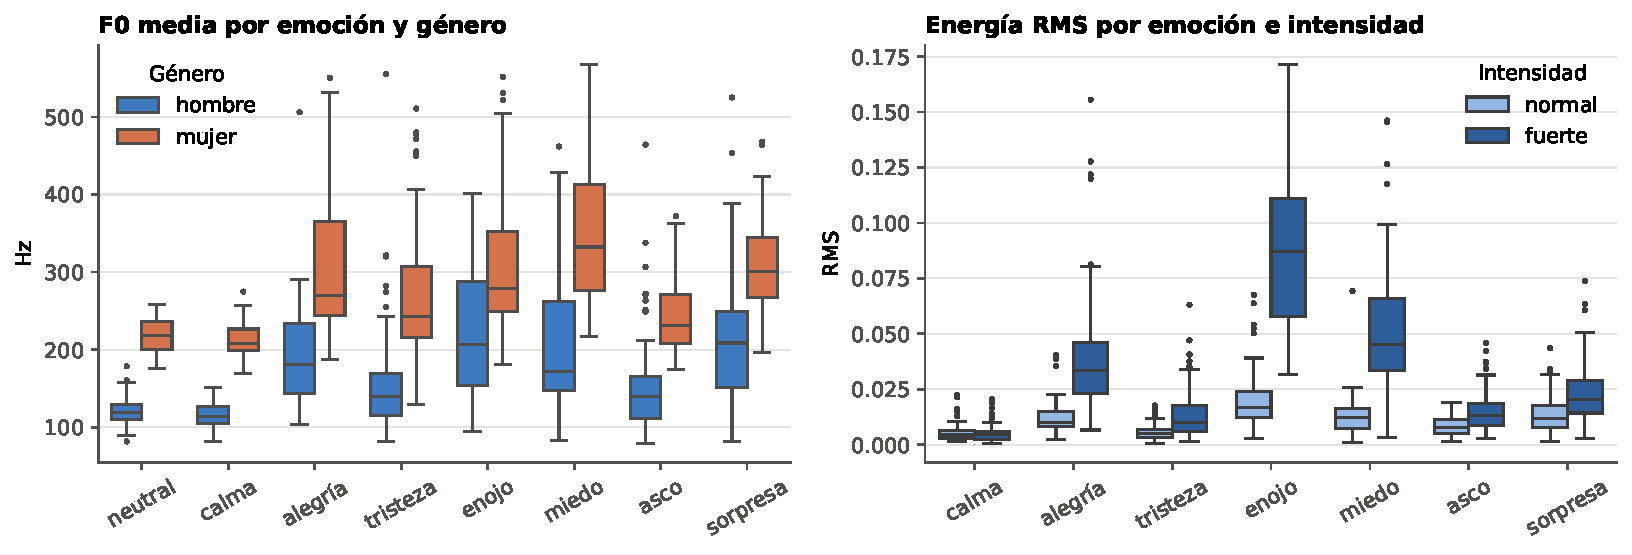
\includegraphics[width=\linewidth]{genero_intensidad}
\caption{Izquierda: F0 media por emoción y género. Derecha: energía RMS por emoción e intensidad.}
\label{fig:genint}
\end{figure}

\subsection{Valores atípicos por género}

Siguiendo la regla IQR por género (\nMujer{} clips de mujeres y \nHombre{} de hombres), la
Tabla~\ref{tab:atipicos} muestra que la energía RMS concentra la mayoría de los valores atípicos:
\(\approx\)10\,\% de los clips en ambos géneros. El resto de los descriptores no pasa de 2.5\,\%, y MFCC1
prácticamente no tiene atípicos.

\begin{table}[H]
\centering
\caption{Valores atípicos (regla IQR) por descriptor y género.}
\label{tab:atipicos}
\small
\begin{tabular}{@{}lrrrr@{}}
\toprule
 & \multicolumn{2}{c}{Mujeres ($n=\nMujer$)} & \multicolumn{2}{c}{Hombres ($n=\nHombre$)} \\
Descriptor & Atípicos & \% & Atípicos & \% \\
\midrule
\tablaAtipicos
\bottomrule
\end{tabular}
\end{table}

\begin{figure}[H]
\centering
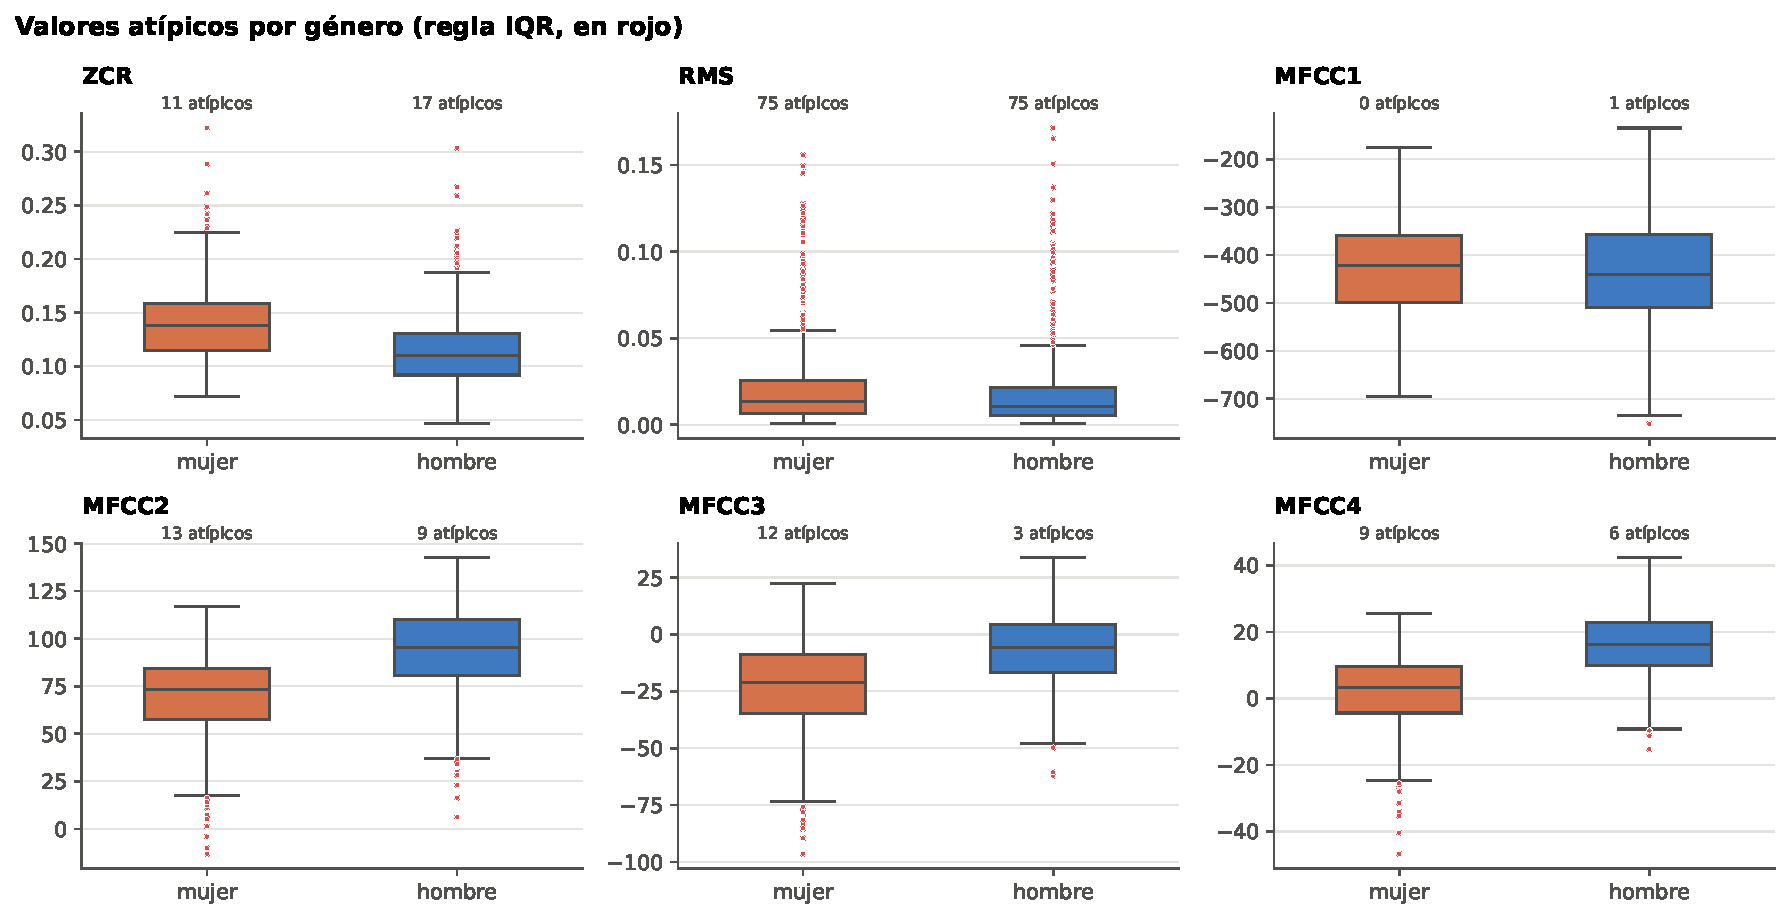
\includegraphics[width=\linewidth]{atipicos_genero}
\caption{Distribución de cada descriptor por género; en rojo, los valores atípicos.}
\label{fig:atipicos}
\end{figure}

La Figura~\ref{fig:atipicosemo} muestra de qué emociones provienen. Los atípicos de RMS son casi todos de
enojo, miedo y alegría, es decir, clips de alta activación con intensidad fuerte. Por lo tanto,
\textbf{no son errores de medición sino el extremo legítimo de esas emociones}, y eliminarlos quitaría
justamente los ejemplos más característicos. Conviene conservarlos y usar transformaciones robustas, como
el logaritmo de la energía o el escalado por cuantiles. La distribución de RMS es muy asimétrica, con una
cola larga a la derecha.

\begin{figure}[H]
\centering
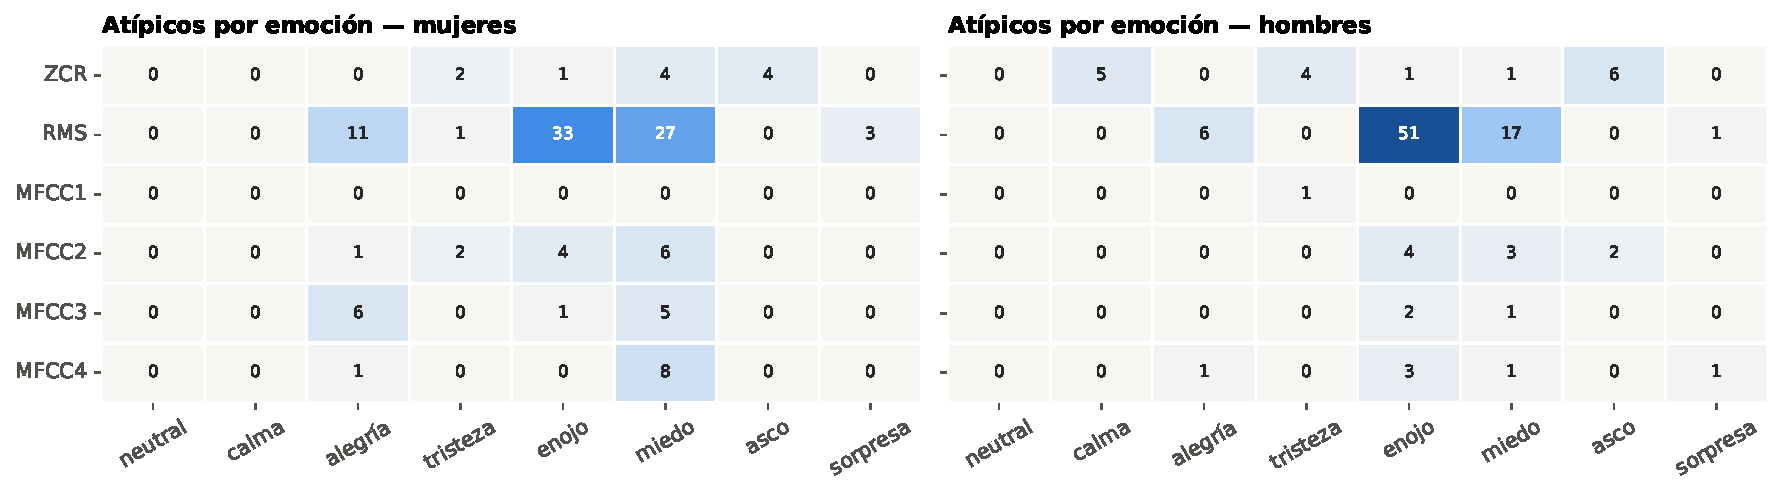
\includegraphics[width=\linewidth]{atipicos_por_emocion}
\caption{Número de valores atípicos por descriptor y emoción, para cada género.}
\label{fig:atipicosemo}
\end{figure}

\subsection{Patrones por emoción y género (gráficos de radar)}

Los gráficos de radar (Figuras~\ref{fig:radarm} y~\ref{fig:radarh}) muestran el perfil medio de cada
emoción en ocho descriptores. Se normalizan con Min-Max dentro de cada género, de modo que 0 corresponde a
la emoción con el valor más bajo y 1 a la más alta. Esto elimina la diferencia absoluta de tono entre
mujeres y hombres y permite comparar la \emph{forma} de los perfiles.

\begin{itemize}
  \item \textbf{Baja activación} (neutral, calma, tristeza): RMS bajo y F0 y centroide bajos o intermedios, con el peso puesto
        en MFCC~2--4, es decir, un espectro con menos energía en frecuencias altas.
  \item \textbf{Enojo}: máximo en RMS y MFCC1 y valores altos en ZCR y centroide, en ambos géneros; es el
        perfil más extremo.
  \item \textbf{Miedo}: F0 y centroide altos. En mujeres además es muy energético (RMS 0.80 frente a 0.40
        en hombres).
  \item \textbf{Asco}: la ZCR más alta con energía baja. Este patrón sugiere una voz más ruidosa o
        fricativa, no más fuerte, y es el que más distingue a asco del resto.
  \item \textbf{Alegría y sorpresa}: F0 alta con energía intermedia. Su parecido explica que se confundan
        entre sí.
\end{itemize}
Los perfiles son muy similares entre géneros. Esto indica que, una vez descontado el tono propio del
hablante, los patrones emocionales son compartidos, lo que respalda normalizar por hablante.

\begin{figure}[H]
\centering
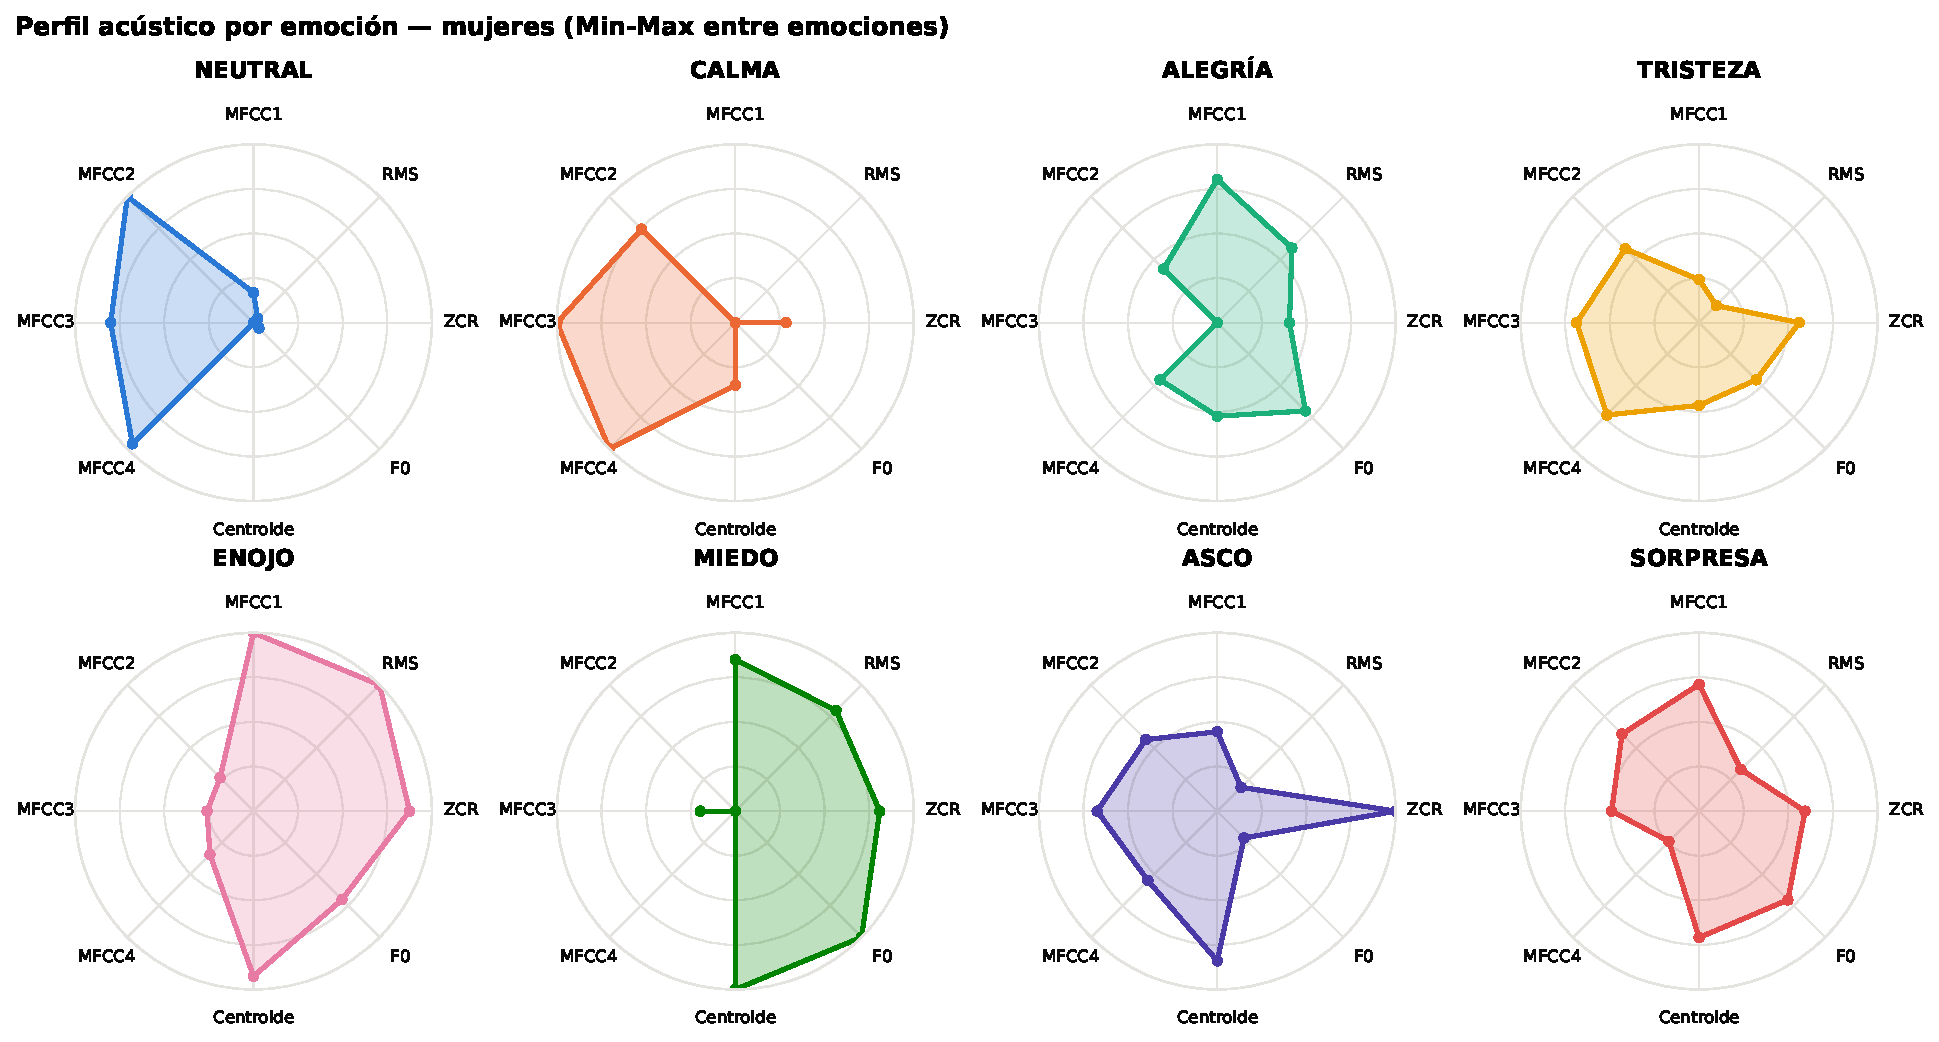
\includegraphics[width=\linewidth]{radar_mujeres}
\caption{Perfil acústico por emoción, mujeres (media por emoción normalizada con Min-Max).}
\label{fig:radarm}
\end{figure}

\begin{figure}[H]
\centering
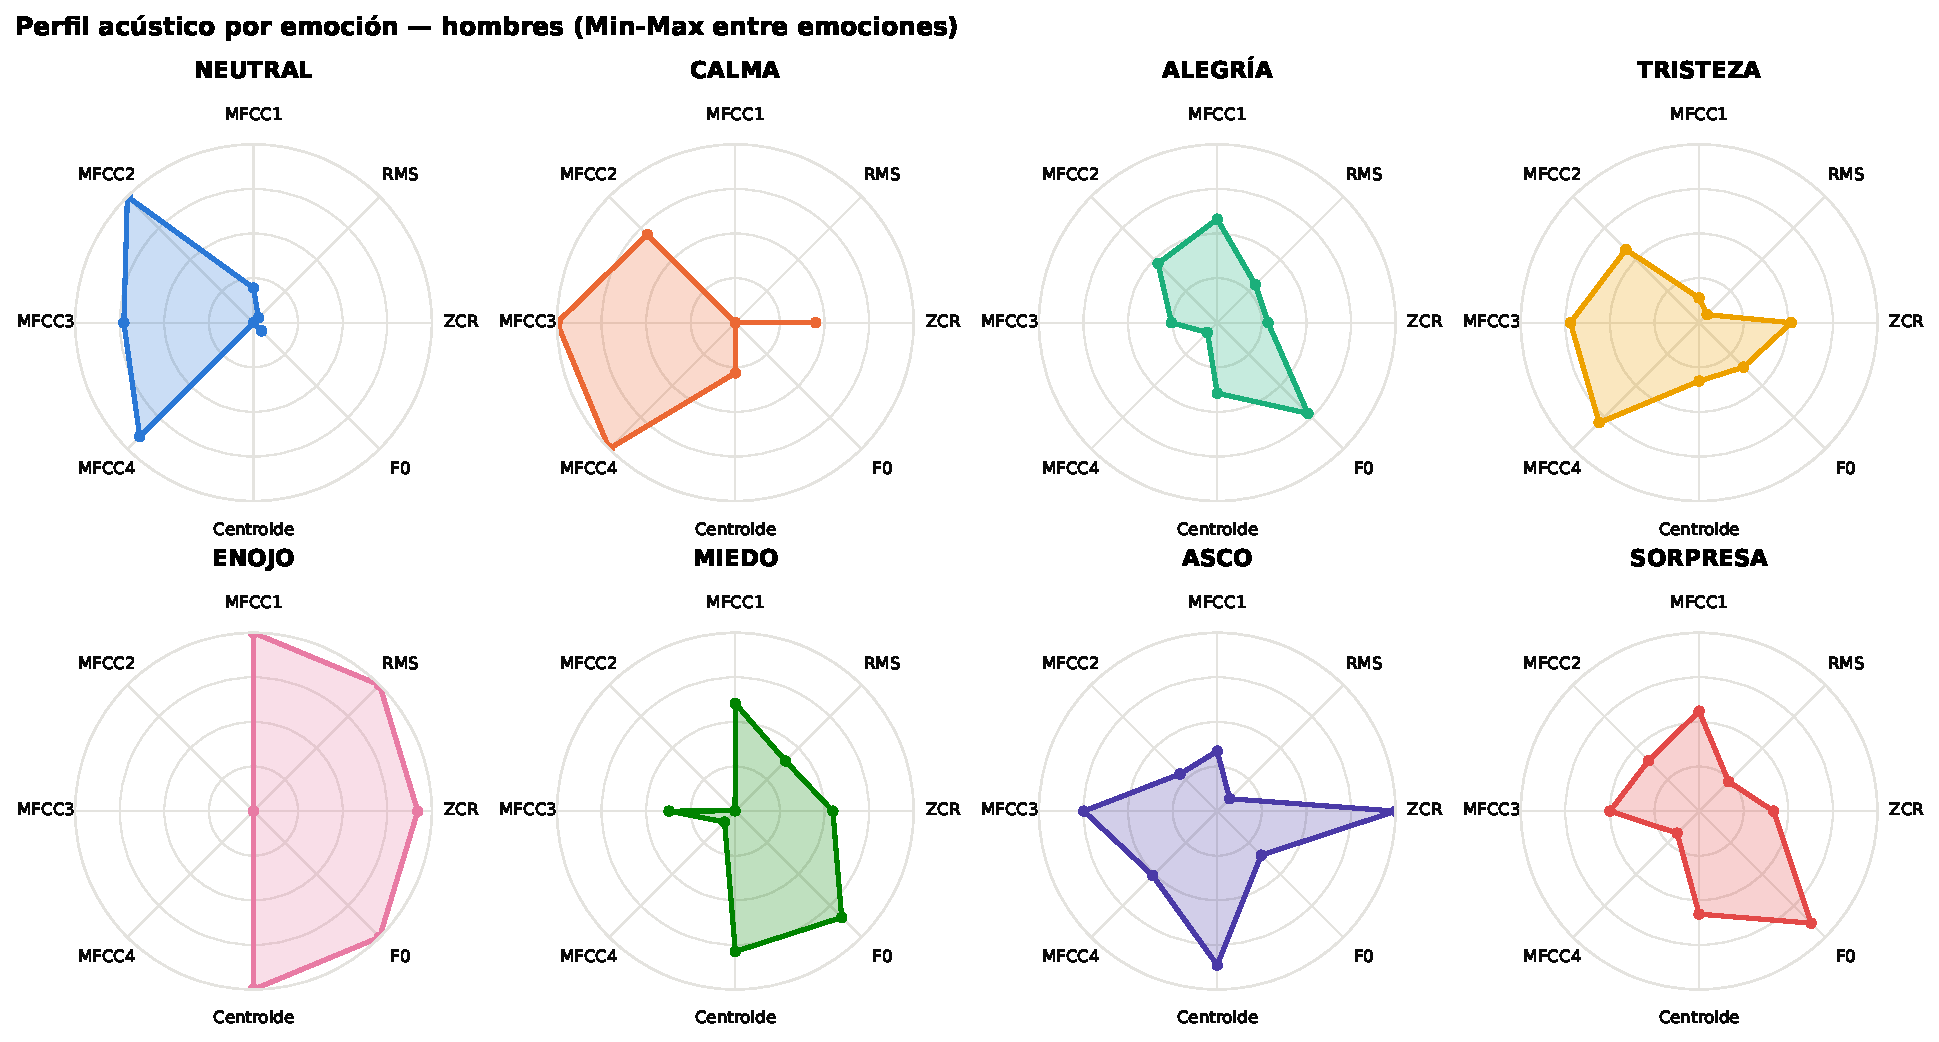
\includegraphics[width=\linewidth]{radar_hombres}
\caption{Perfil acústico por emoción, hombres (media por emoción normalizada con Min-Max).}
\label{fig:radarh}
\end{figure}

\subsection{Perfil MFCC}

Los MFCC describen la envolvente espectral, es decir, el timbre. El primer coeficiente sigue a la energía
($\rho=0.97$ con la RMS): es alto en enojo y bajo en calma, neutral y tristeza. Los coeficientes 2 a 6
distinguen a las emociones de baja activación, con valores positivos en neutral y calma, de las de alta
activación, con valores negativos en enojo y miedo. Los coeficientes de orden alto (15--20) aportan menos
contraste, salvo en miedo (Figura~\ref{fig:mfcc}).

\begin{figure}[H]
\centering
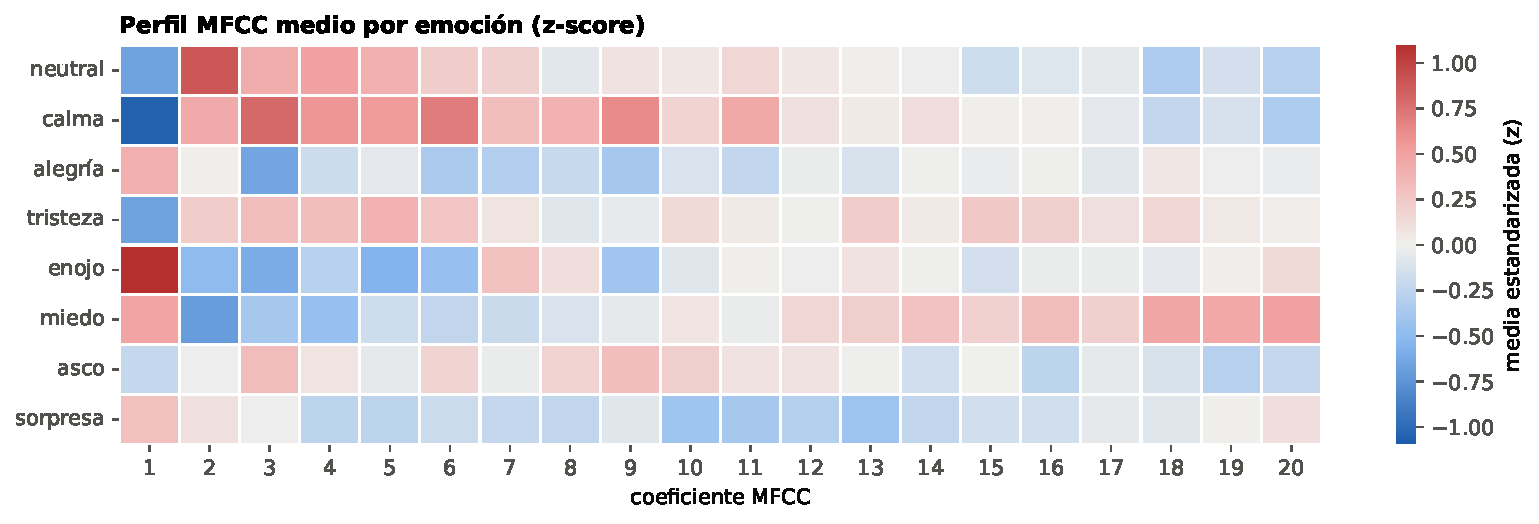
\includegraphics[width=\linewidth]{mfcc_por_emocion}
\caption{Media estandarizada (z) de cada coeficiente MFCC por emoción.}
\label{fig:mfcc}
\end{figure}

\subsection{Redundancia entre descriptores}

Varios descriptores son casi redundantes (Figura~\ref{fig:corr}): RMS y MFCC1 ($\rho=0.97$), centroide y
\emph{roll-off} ($\rho=0.93$), desviación y rango de F0 ($\rho=0.99$), y ZCR y centroide ($\rho=0.87$).
Por ello conviene usar regularización o reducción de dimensión al combinar descriptores agregados.

\begin{figure}[H]
\centering
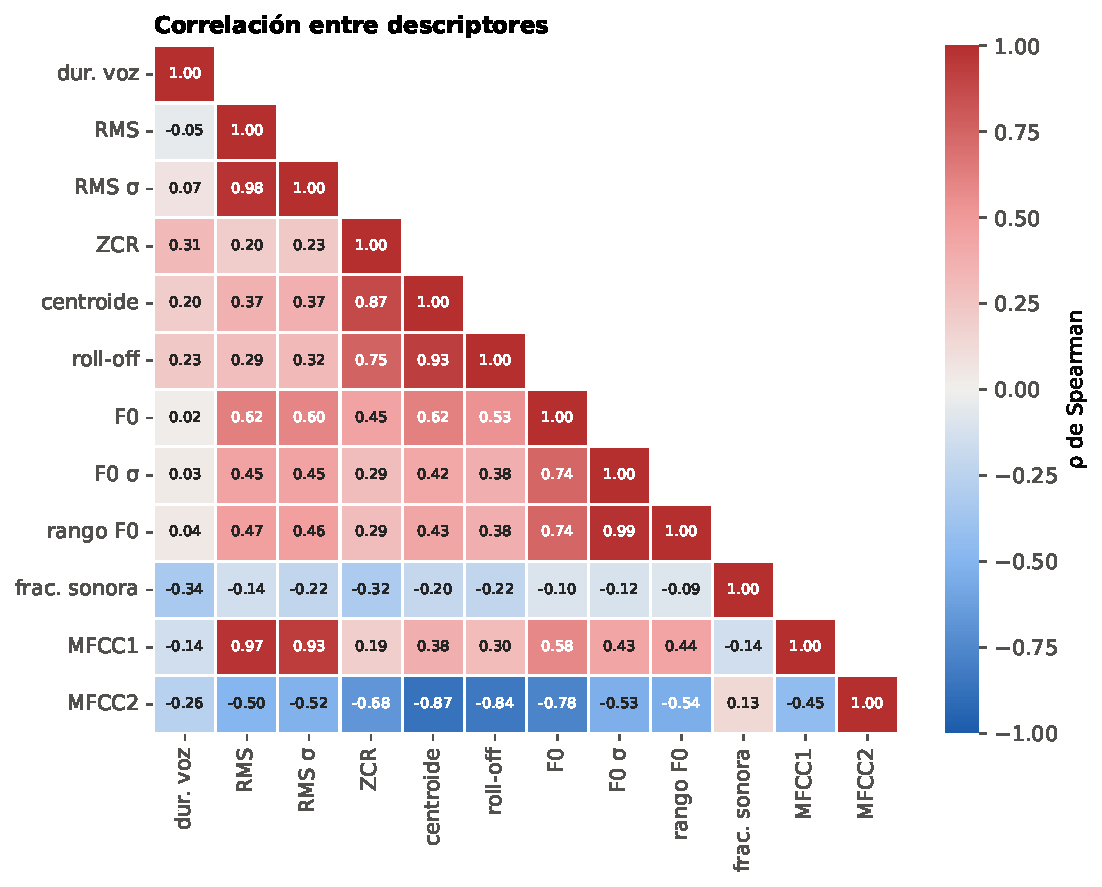
\includegraphics[width=.72\linewidth]{correlacion_descriptores}
\caption{Correlación de Spearman entre descriptores.}
\label{fig:corr}
\end{figure}

\subsection{Estructura global: emoción frente a hablante}

En el PCA (Figura~\ref{fig:pca}), las dos primeras componentes explican \pcUno\,\% y \pcDos\,\% de la
varianza, y se requieren \nPCNoventa{} componentes para alcanzar el 90\,\%. La primera componente actúa
como un eje de \emph{activación}: neutral, calma y tristeza se ubican de un lado, y enojo, miedo y alegría
del otro. Aun así, el traslape entre emociones es considerable.

\begin{figure}[H]
\centering
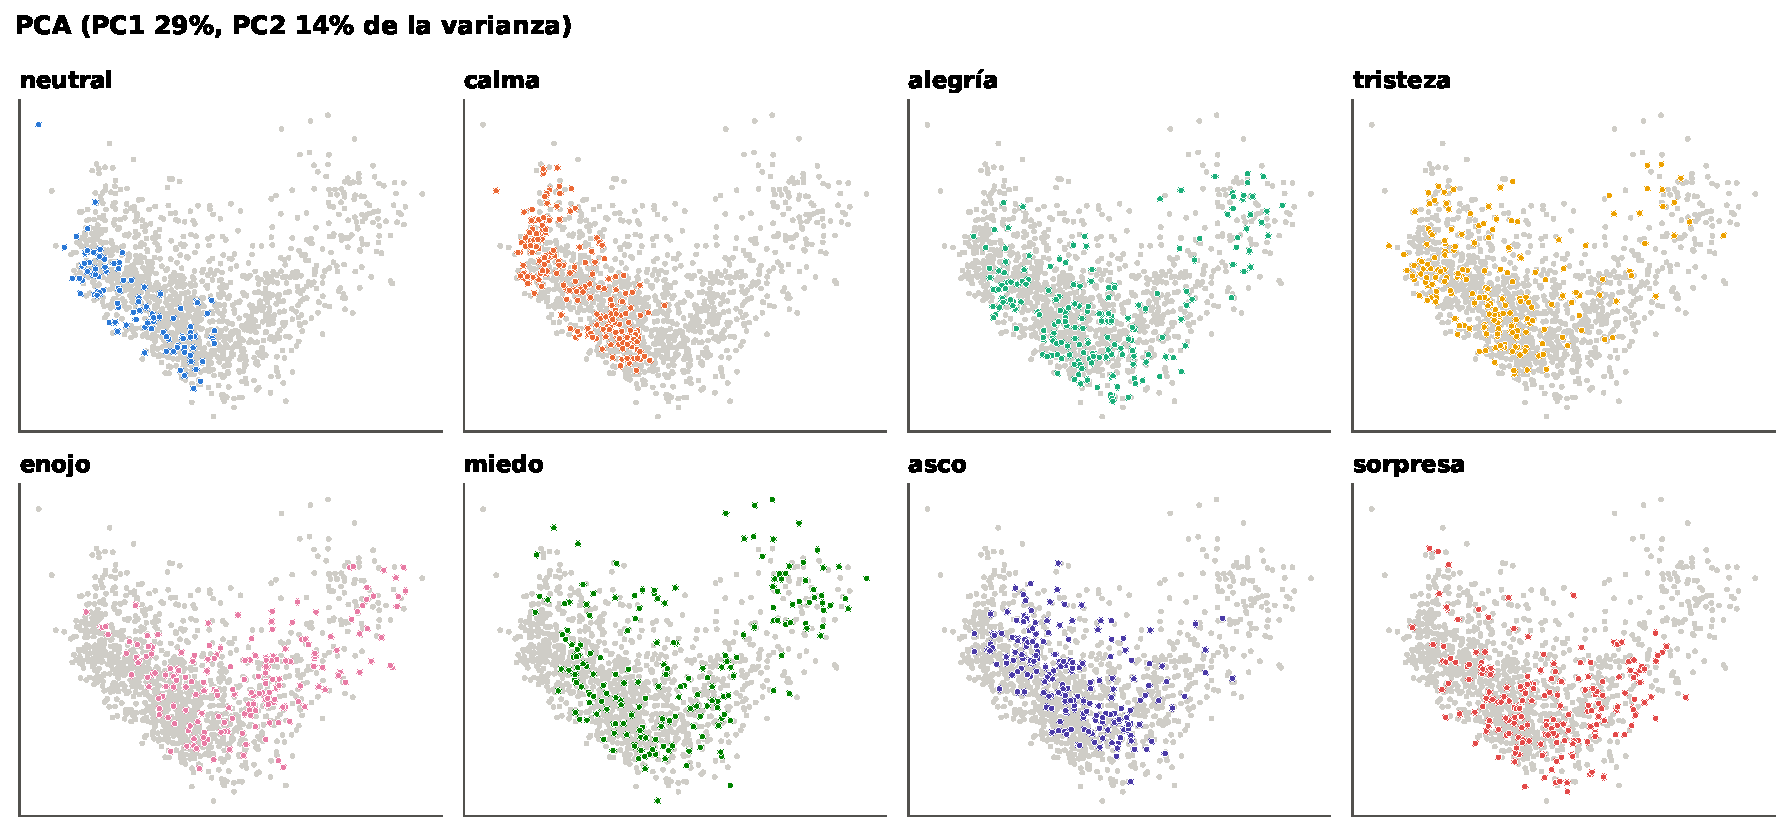
\includegraphics[width=\linewidth]{pca_emociones}
\caption{PCA de los descriptores; cada panel resalta una emoción sobre el resto (gris).}
\label{fig:pca}
\end{figure}

El t-SNE confirma este traslape: las emociones no forman grupos compactos (Figura~\ref{fig:tsne}). En
cambio, el mismo mapa coloreado por género muestra dos regiones casi disjuntas
(Figura~\ref{fig:tsnegen}). Por tanto, \textbf{la variación entre hablantes domina sobre la variación
emocional} en el espacio de descriptores.

\begin{figure}[H]
\centering
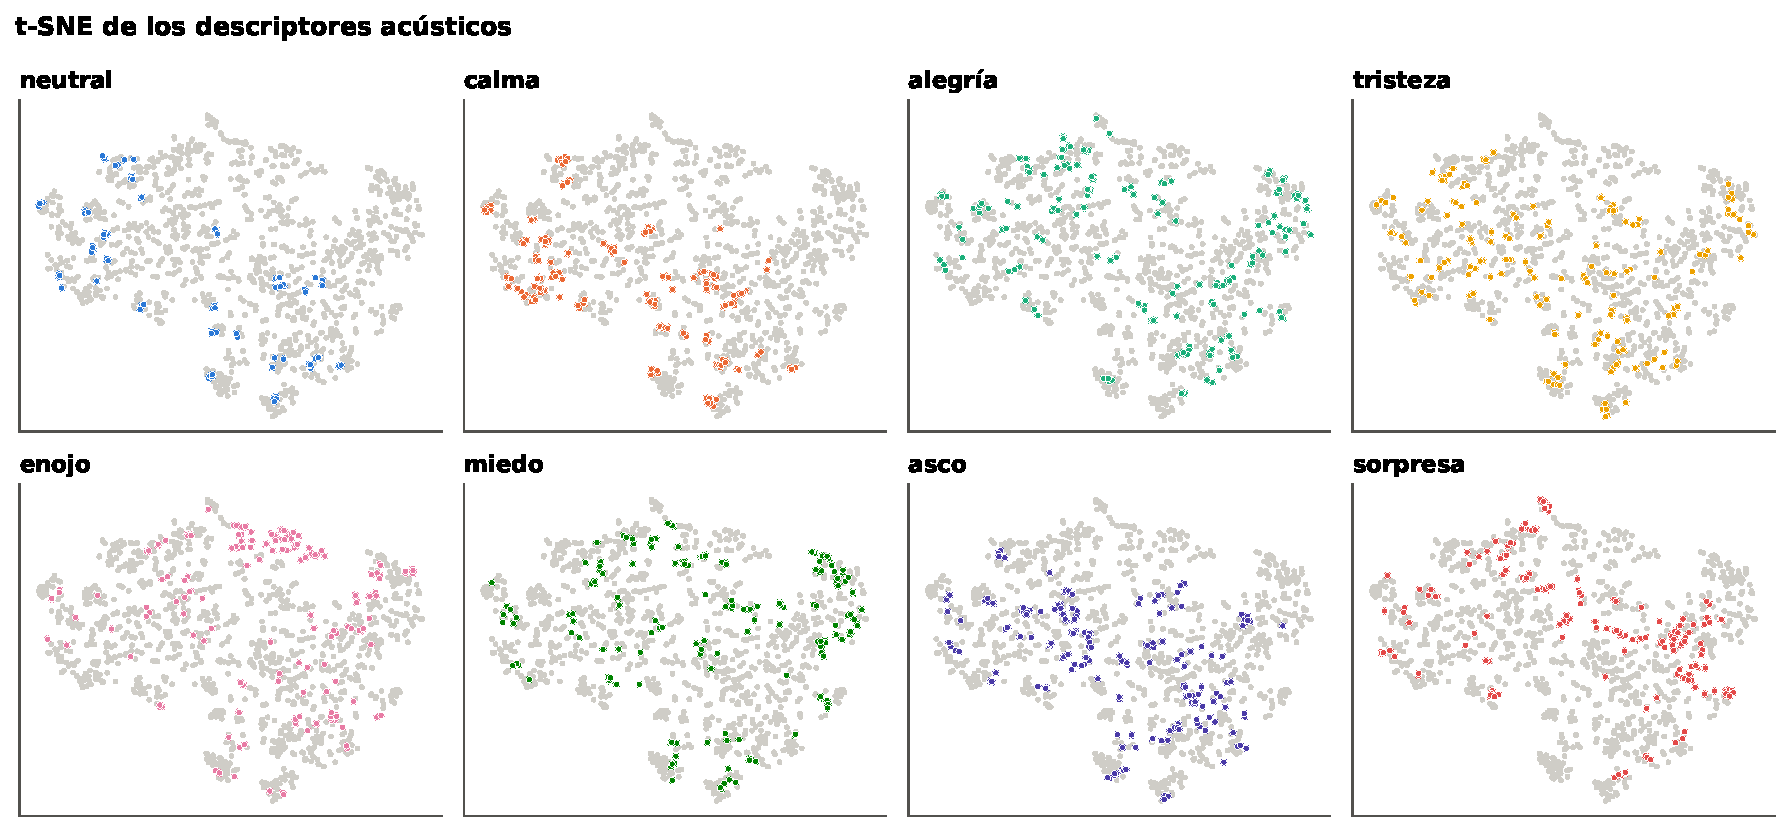
\includegraphics[width=\linewidth]{tsne_emociones}
\caption{t-SNE de los descriptores acústicos; cada panel resalta una emoción.}
\label{fig:tsne}
\end{figure}

\begin{figure}[H]
\centering
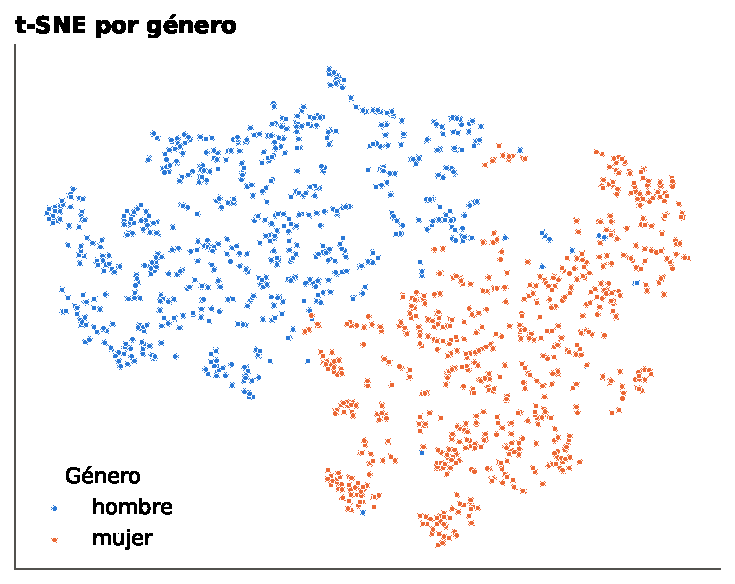
\includegraphics[width=.5\linewidth]{tsne_genero}
\caption{El mismo t-SNE coloreado por género del hablante.}
\label{fig:tsnegen}
\end{figure}

\section{Conclusiones}

\begin{enumerate}[label=\arabic*.]
  \item El corpus está completo y es limpio: \nClips{} clips sin duplicados ni nulos. Solo requiere
        convertir \nEstereo{} clips estéreo a mono y recortar silencios, que ocupan \(\approx\)50\,\% de
        cada clip.
  \item Está balanceado por actor y género. La clase neutral tiene la mitad de muestras que el resto, por
        lo que conviene reportar métricas macro y considerar pesos por clase.
  \item Energía, F0, duración y centroide espectral difieren significativamente entre emociones. Juntos
        describen sobre todo un eje de activación (alta frente a baja). Las emociones con activación
        similar, como enojo y alegría o calma y neutral, son las que más se traslapan.
  \item Los valores atípicos (regla IQR) se concentran en la energía, con \(\approx\)10\,\% de los clips
        por género, y provienen de enojo, miedo y alegría con intensidad fuerte. Son señal, no ruido: se
        recomienda conservarlos y usar escalas robustas.
  \item Los gráficos de radar muestran perfiles por emoción casi iguales en mujeres y hombres una vez
        normalizados. Destacan la energía en enojo, el tono en miedo y sorpresa, y la ZCR en asco.
  \item La frame length de \frameLen{} y la hop length de \hopLen{} muestras equilibran la resolución
        temporal y la estabilidad de MFCC, ZCR y RMS, y coinciden con el modelo de referencia.
  \item La identidad y el género del hablante son la principal fuente de variación. En consecuencia, la
        evaluación del modelo debe reservar actores completos para prueba (evaluación independiente del
        hablante), y conviene normalizar por hablante o aumentar los datos con variaciones de tono.
  \item Los datos quedan disponibles en Supabase con acceso público de solo lectura, lo que permite
        reproducir el análisis desde cualquier equipo sin copias locales.
\end{enumerate}

\begin{thebibliography}{9}
\bibitem{livingstone2018}
S.~R. Livingstone y F.~A. Russo, ``The Ryerson Audio-Visual Database of Emotional Speech and Song
(RAVDESS): A dynamic, multimodal set of facial and vocal expressions in North American English'',
\emph{PLoS ONE}, 13(5): e0196391, 2018. \url{https://doi.org/10.1371/journal.pone.0196391}.
Licencia CC BY-NC-SA 4.0.

\bibitem{mcfee2015}
B.~McFee \emph{et al.}, ``librosa: Audio and music signal analysis in Python'', en \emph{Proc. 14th
Python in Science Conference}, pp.~18--25, 2015.

\bibitem{kaggleref}
gemmin, ``Speech Emotion Recognition 90\%'', Kaggle Notebook.
\url{https://www.kaggle.com/code/gemmin/speech-emotion-recognition-90/notebook}.
\end{thebibliography}

\end{document}
